\chapter{Implementacja}
\label{cha:implementacja}
Rozdział opisuje technologie użyte w~pracy oraz przedstawia strukturę bazy danych i~implementacje wydzielonych komponentów. Aplikacja prezentowana jest od strony implementacyjnej. 

%---------------------------------------------------------------------------
\section{Stos technologiczny}
\label{sec:stosTechnologiczny}
Rysunek~\ref{fig:technologyStack} prezentuje technologie użyte podczas implementacji projektu. Stos przedstawiony na rysunku został podzielony na część związaną z~interfejsem użytkownika oraz na część związaną z~serwerem. Dodatkowo pokazana jest technologia, która została wybrana jako zewnętrzny system i~zintegrowana z~aplikacją ,,DAR''. Kolejne podrozdziały pogłębiają temat wybranych technologii.
\begin{figure}
    \centering
    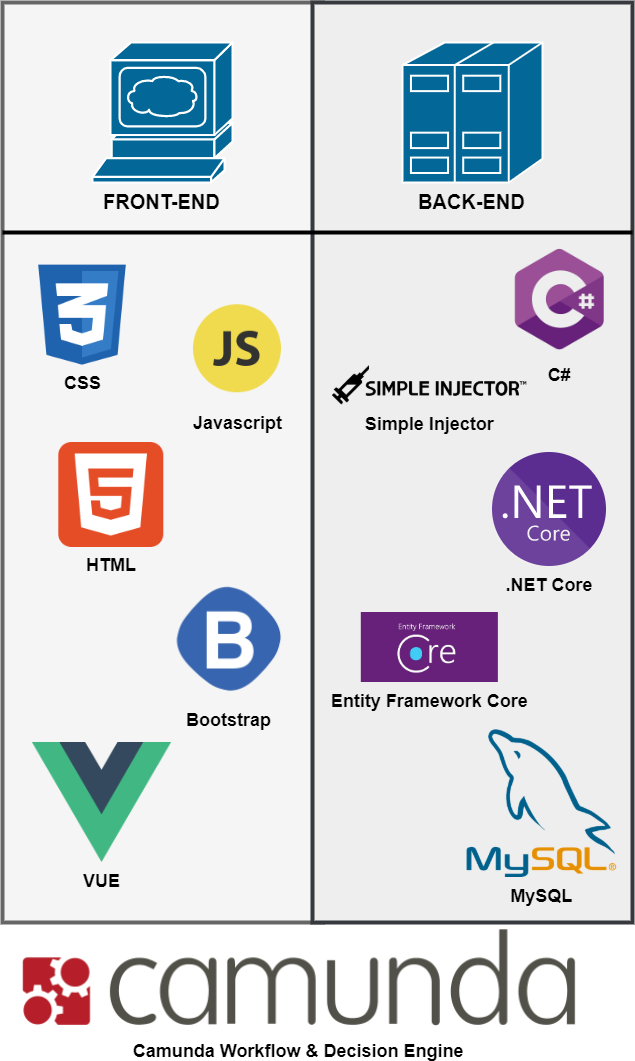
\includegraphics[width=\textwidth, height=0.4\textheight,keepaspectratio]{./assets/technologyStack.png}
    \caption{Stos technologiczny aplikacji ,,DAR''}
    \label{fig:technologyStack}
\end{figure} 

%---------------------------------------------------------------------------
\subsection{Technologie front-end}
\label{sec:frontEndTechnologie}
Przedstawione technologie po stronie lewej rysunku~\ref{fig:technologyStack} są związane z~interfejsem użytkownika. Występuje tutaj podział na języki programowania oraz szkielety aplikacyjne/biblioteki:
\begin{itemize}
    \item \textbf{Języki programowania/Języki komputerowe}
    \begin{itemize}
        \item \textbf{Javascript} -- interpretowany, dynamiczny język programowania wykorzystywany jako główny język skryptowy na stronach internetowych. Według ankiety~\cite{StackSurvey} z~2019 roku, przeprowadzonej na serwisie \emph{StackOverflow}\footnote{Jeden z~najpopularniejszych serwisów dla programistów: \url{https://stackoverflow.com/}.} jest to obecnie najpopularniejszy język świata, bezsprzecznie królujący w~świecie przeglądarek internetowych.
        \item \textbf{HTML} -- \emph{HyperText Markup Language} to język komputerowy stworzony w~celu tworzenia stron internetowych. Umożliwia tworzenie nagłówków, połączeń, ustrukturyzowanych sekcji, paragrafów i wiele innych elementów...
        \item \textbf{CSS} -- \emph{Cascading Style Sheets} to język związany ze stylem dokumentów. Umożliwia on specyfikację, jak pliki są prezentowane użytkownikom -- określa ich styl, ułożenie elementów oraz inne atrybuty. Najczęściej używany razem z~językiem \emph{HTML}. 
    \end{itemize}
    \newpage
    \item \textbf{Szkielety aplikacyjne/Biblioteki}
    \begin{itemize}
        \item \textbf{Bootstrap} -- otwarte oprogramowanie, będące biblioteką \emph{CSS}, nad którą piecze sprawują programiści \emph{Twittera}\footnote{Jeden z~najpopularniejszych portali społecznościowych: \url{https://twitter.com/}.}. Bootstrap usprawnia tworzenie aplikacji internetowych, udostępniając wiele szablonów \emph{HTML} oraz \emph{CSS}, które upiększają stronę.
        \item  \textbf{Vue} -- Szkielet aplikacyjny front-end napisany w~JavaScript, do tworzenia wszelkiego rodzaju interfejsów użytkownika w~tym \emph{Single Page Application}. Usprawnia tworzenie aplikacji internetowych poprzez udostępnienie wielu funkcjonalności, w~tym chociażby manipulowanie drzewem obiektów dokumentu, co pozwala na dynamiczne podmienianie danych na stronie bez konieczności pełnego przeładowania strony. Jest on bardzo podobny do najpopularniejszych szkieletów aplikacyjnych, takich jak \emph{React}\footnote{Więcej na temat \emph{React}: \url{https://pl.reactjs.org/}.} lub \emph{Angular}\footnote{Więcej na temat \emph{Angular}: \url{https://angular.io/}.}. Według wspomnianej już ankiety~\cite{StackSurvey}, \emph{Vue} zyskuje bardzo szybko na popularności.  
    \end{itemize}
\end{itemize}

%---------------------------------------------------------------------------
\subsection{Technologie back-end}
\label{sec:backEndTechnologie}
Przedstawione technologie po stronie prawej rysunku~\ref{fig:technologyStack} są związane z~warstwą logiki oraz danych. Występuje tutaj podział na języki programowania, szkielety aplikacyjne/biblioteki oraz oprogramowania do zarządzania bazą danych:
\newpage
\begin{itemize}
    \item \textbf{Języki programowania}
        \begin{itemize}
            \item \textbf{C\#} -- wysokopoziomowy, obiektowy język programowania. Był on odpowiedzią \emph{Microsoftu}\footnote{Jedna z~największych korporacji świata: \url{https://www.microsoft.com}.} na język \emph{Java}\footnote{Jeden z~najbardziej popularnych, obiektowych języków programowania na świecie: \url{https://www.java.com}.}, ściśle zintegrowany z~platformą \emph{Microsoftu .NET}. Wcześniej używany głównie do tworzenia aplikacji na systemy \emph{Windows}, ale odkąd powstał wieloplatformowy \emph{.NET Core} sytuacja uległa zmianie. Często używany do tworzenia internetowych \emph{API} oraz aplikacji mobilnych dzięki technologi \emph{Xamarin}. Przykładem aplikacji stworzonej przy użyciu C\# jest portal \emph{StackOverflow}.
        \end{itemize}
    \item \textbf{Szkielety aplikacyjne/Biblioteki}
    \begin{itemize}
        \item \textbf{.NET Core} -- a~właściwie \emph{ASP .NET Core}, jest to otwarte oprogramowanie, będące wieloplatformowym szkieletem aplikacyjnym rozwijanym przez \emph{Microsoft} do tworzenia wysoko wydajnych, nowoczesnych, opartych na technologi chmurowej, internetowo połączonych aplikacji. Cały kod tego projektu dostępny jest na platformie \emph{GitHub}\footnote{Zobacz: \url{https://github.com/aspnet/AspNetCore}.}. Dodatkowo dzięki wieloplatformowości umożliwia on tworzenie oraz działanie na platformach, takich jak \emph{Linux} czy \emph{macOS}, a~oprócz tego jest on stworzony z~myślą o konteneryzacji. \emph{ASP .NET Core} wspiera najlepsze metodyki tworzenia aplikacji poprzez promowanie modularności, wbudowane mechanizmy wstrzykiwania zależności czy wsparcie dla rozwiązań chmurowych oraz \emph{gRPC}\footnote{Więcej na temat gRpc: \url{https://grpc.io/}.}. Szkielet aplikacyjny \emph{.NET Core} w~cytowanej już ankiecie~\cite{StackSurvey} portalu \emph{StackOverflow} z~roku 2019, zyskał pierwsze miejsce w~rankingu najlepszych szkieletów aplikacyjnych. Natomiast pod względem wydajności plasuje się w~czołówce (miejsce 10) według rankingu \emph{TechEmpower}~\cite{WebBenchmark}, wyprzedzając takie szkielety aplikacyjne jak \emph{Django} (miejsce 213), \emph{Spring} (miejsce 245), czy \emph{Ruby on Rails} (miejsce 215).
        \item \textbf{Entity Framework Core} -- jest to ORM (\emph{Object-Relational Mapper}), czyli narzędzie pozwalające programistom działać z~danymi w~stylu obiektowym. Jego głównym zadaniem jest mapowanie obiektów zdefiniowanych w~aplikacji w~wybranym języku programowania, do danych przechowywanych w~relacyjnej bazie danych. Narzędzie to bardzo ułatwia pracę z~bazą danych, ukrywając za abstrakcjami połączenia z~bazą danych, wszelkie konwersje do języka \emph{SQL} oraz tworzenie struktur bazy danych.
        \item \textbf{Simple Injector} -- biblioteka służąca jako kontener wstrzykiwania zależności. Szkielet aplikacyjny \emph{.NET Core} posiada wbudowane narzędzie do wstrzykiwania zależności jednak \emph{Simple Injector} działa opierając się na nim i~rozbudowując jego możliwości. Jego głównym zadaniem jest pilnowanie oraz zarządzanie cyklem życia obiektów w~aplikacji, poprzez zastosowanie odwrócenia sterowania~\cite{DI}.
    \end{itemize}
    \newpage
    \item \textbf{Oprogramowanie do zarządzania bazą danych}
        \begin{itemize}
            \item \textbf{MySQL} -- jest to otwarte oprogramowanie, będące systemem do zarządzania relacyjnymi bazami danych, opierającym się na modelu klient-serwer. Odpowiada on za stworzenie bazy danych i~odpowiednie przechowywanie oraz zarządzanie informacjami. Komunikacja opiera się na języku SQL (\emph{Structured Query Language}), służącym do manipulowania danymi.
        \end{itemize}
\end{itemize}

%---------------------------------------------------------------------------
\subsection{Zewnętrzny System}
\label{sec:zewnętrznySystem}
\emph{Camunda} została wybrana jako zewnętrzny system do zarządzania modelami procesów oraz decyzji. Jest to otwarte oprogramowanie napisane w języku \emph{Java}, pozwalające na uruchomienie wykonywalnych modeli procesów, ewaluację decyzji oraz monitorowanie całego przepływu działań procesu. Najważniejsze komponenty, które udostępnia \emph{Camunda} w~kontekście niniejszej pracy to:
\begin{itemize}
    \item \textbf{Silnik}
        \begin{itemize}
            \item \textbf{Process Engine} -- silnik napisany w~języku \emph{Java}, umożliwiający uruchamianie procesów w~notacji \emph{BPMN} oraz decyzji w~notacji \emph{DMN}.
        \end{itemize}
    \item \textbf{Aplikacje internetowe}
        \begin{itemize}
            \item \textbf{REST API} -- \emph{API} umożliwiające dostęp do wspomnianego wcześniej silnika oraz platformy zarządzającej procesami i~decyzjami. Głównie wykorzystywane w~celu wdrożenia modelów \emph{BPMN} oraz \emph{DMN} do platformy.
            \item \textbf{Camunda Tasklist} -- część platformy do zarządzania procesami i~decyzjami. Umożliwia uruchomienie procesu oraz wykonywanie zadań użytkownika, np. podanie odpowiednich danych, potrzebnych do działania procesu.
            \item \textbf{Camunda Cockpit} -- część platformy do zarządzania procesami i~decyzjami. Umożliwia obserwację i~edycję modeli \emph{BPMN} oraz \emph{DMN}, oraz monitorowanie wykonywanych procesów i~ewaluowanych decyzji.
        \end{itemize}
\end{itemize}

Pomimo że \emph{Camunda} jest w~wersji podstawowej otwartym oprogramowaniem, w~kontekście niniejszej pracy wymagana jest edycja typu \emph{Enterprise} będąca wersją płatną. Wynika to z~faktu, że modele \emph{DMN} tworzone przez aplikację \emph{DAR} nie są wypełnione regułami -- ze względu na brak takowych w~diagramach \emph{ARD}. W utworzonych tabelach decyzyjnych należy uzupełnić reguły, tak aby decyzje mogły być ewaluowane. Ta możliwość jest udostępniona tylko w~wersji płatnej.

%---------------------------------------------------------------------------
\section{Schemat bazy danych}
\label{sec:schematBazyDanych}
Dzięki wspomnianemu wcześniej \emph{Entity Framework Core}, wszystkie klasy, które zostały zmapowane ze schematu pliku \emph{HML} do kodu w~języku \emph{C\#}, automatycznie zostały użyte do budowy tabel w~relacyjnej bazie danych. Rysunek~\ref{fig:databaseScheme} przedstawia efekt tego zabiegu. 
\begin{figure}
    \centering
    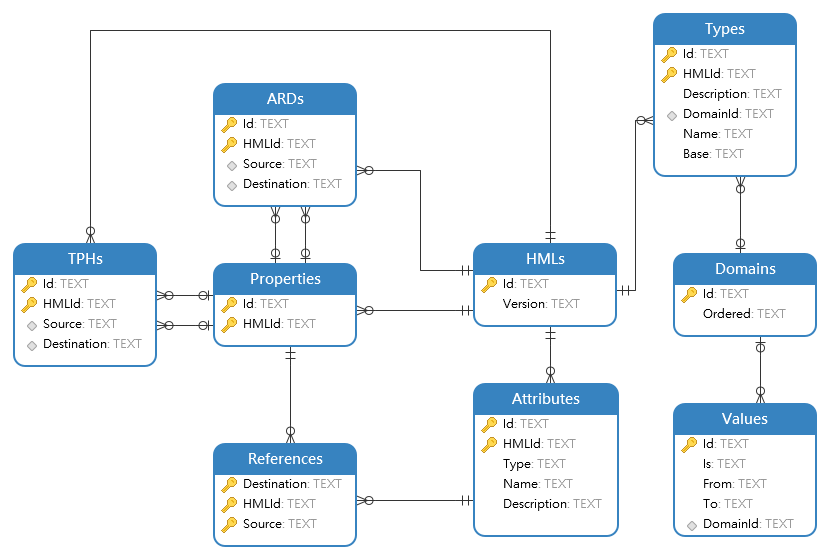
\includegraphics[width=\textwidth,height=0.4\textheight,keepaspectratio]{./assets/databaseScheme.png}
    \caption{Schemat bazy danych aplikacji ,,DAR''}
    \label{fig:databaseScheme}
\end{figure}

Warto przyjrzeć się bliżej poszczególnym tabelom:
\begin{itemize}
    \item \textbf{Tabela HMLs} -- serce całego schematu. Posiada jeden klucz główny \emph{Id}, identyfikujący poszczególne pliki \emph{HML}. Dodatkowo określa wersję danego pliku.
    \item \textbf{Tabela Properties} -- reprezentuje właściwości opisane w~plikach. Posiada dwa klucze, jeden główny, będący złożeniem \emph{Id} oraz \emph{HMLId}, służący do identyfikacji, oraz drugi obcy \emph{HMLId}, będący połączeniem do tabeli \emph{HMLs}.
    \item \textbf{Tabela Attributes} -- reprezentuje atrybuty opisane w~plikach. Posiada dwa klucze, jeden główny, będący złożeniem \emph{Id} oraz \emph{HMLId}, służący do identyfikacji, oraz drugi obcy \emph{HMLId}, będący połączeniem do tabeli \emph{HMLs}. Zawiera dodatkowo informacje o atrybutach, takie jakie nazwa, opis oraz typ danych.
    \item \textbf{Tabela References} -- pośredniczy pomiędzy właściwościami, a~atrybutami. Posiada trzy klucze. Jeden podstawowy będący złożeniem \emph{Destination}, \emph{Source} oraz \emph{HMLId}, służący do identyfikacji oraz dwa obce: złożenie \emph{Source} oraz \emph{HMLId}, będące połączeniem do tabeli \emph{Properties} i~złożenie \emph{Destination} oraz \emph{HMLId}, będące połączeniem do tabeli \emph{Attributes}.
    \item \textbf{Tabela Types} -- reprezentuje typy danych opisane w~plikach. Posiada trzy klucze. Jeden podstawowy \emph{Id}, służący do identyfikacji oraz dwa obce: \emph{HMLId} będący połączeniem do tabeli \emph{HMLs} oraz \emph{DomainId}, będący połączeniem do tabeli \emph{Domains}. Dodatkowo określa takie właściwości, jak opis typu, nazwa oraz podstawa (przykładowo numeryczna).
    \item \textbf{Tabela Values} -- reprezentuje możliwe wartości danego typu. Posiada dwa klucze. Jeden podstawowy \emph{Id}, służący do identyfikacji oraz jeden obcy \emph{DomainId}, będący połączenim do tabeli \emph{Domains}. Dodatkowo określa różne możliwości związane z~wartościami, typu przedziały wartości, czy jest to wartość numeryczna lub konkretna wartość.
    \item \textbf{Tabela Domains} -- reprezentuje dziedziny opisane w~pliku i~pośredniczy między tabelami \emph{Types} and \emph{Values}. Posiada jeden klucz główny \emph{Id}, służący do identyfikacji.
    \item \textbf{Tabela ARDs} -- reprezentuje zależności między właściwościami. Posiada cztery klucze: jeden podstawowy złożony z~\emph{Id} oraz \emph{HMLId}, służący do identyfikacji i trzy obce: \emph{HMLId}, będące połączeniem do tabeli \emph{HMLs} oraz dwa złożenia: \emph{HMLId} i~\emph{Source}, będące połączeniem do tabeli \emph{Properties}, do właściwości niezależnej oraz złożenie \emph{HMLId} i~\emph{Destination}, będące połączeniem do tabeli \emph{Properties}, do właściwości zależnej.
    \item \textbf{Tabela TPHs} -- właściwie niewykorzystywana, reprezentuje historię zależności między właściwościami. Posiada cztery klucze: jeden podstawowy złożony z~\emph{Id} oraz \emph{HMLId}, służący do identyfikacji oraz trzy obce: złożenie \newline \emph{HMLId} i~\emph{Source}, będące połączeniem do tabeli \emph{Properties}, do właściwości niezależnej, złożenie \emph{HMLId} i~\emph{Destination}, będące połączeniem do tabeli \emph{Properties}, do właściwości zależnej oraz \emph{HMLId}, będące połączeniem do tabeli \emph{HMLs}.
\end{itemize} 

%---------------------------------------------------------------------------
\section{Schemat klas}
\label{sec:schematKlas}
Rysunek~\ref{fig:classDiagram1} przedstawia najistotniejsze klasy aplikacji. Pominięte zostały klasy związane z~infrastrukturą, określające jak szkielet aplikacyjny \emph{ASP .NET Core} ma obsługiwać przychodzące zapytania \emph{HTTP}, którego serwera lub której bazy danych ma używać. Dodatkowo niezaprezentowane zostały encje, będące prostymi klasami bez żadnej logiki, zawierającymi jedynie pola, gdyż zostały wygenerowane one automatycznie na podstawie specyfikacji plików \emph{ARD}, \emph{BPMN} oraz \emph{DMN}.
\begin{figure}
    \centering
    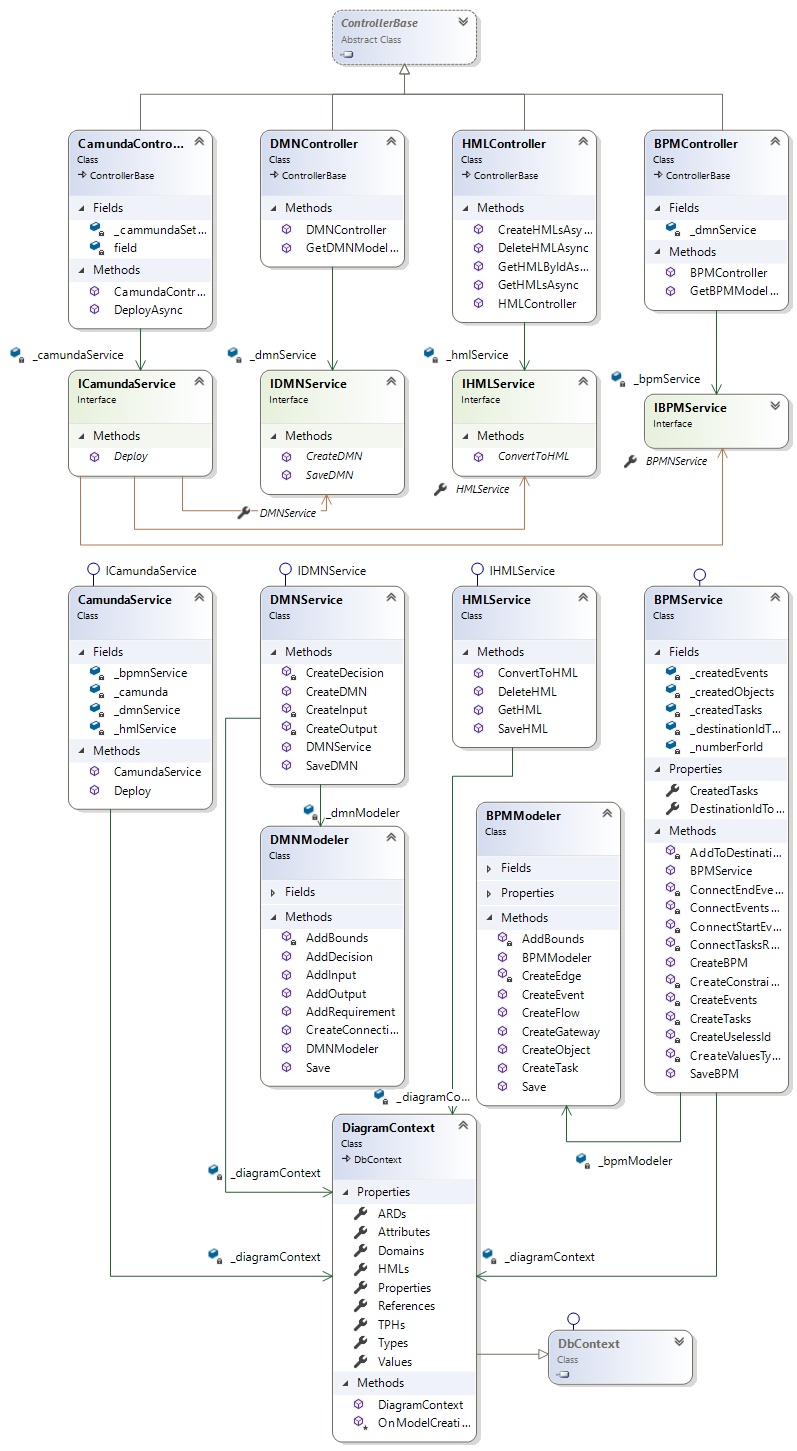
\includegraphics[width=\textwidth, height=0.95\textheight,keepaspectratio]{./assets/classDiagram.png}
    \caption{Schemat klas wchodzących w~skład \emph{REST API} aplikacji ,,DAR''}
    \label{fig:classDiagram1}
\end{figure}

Na rysunku~\ref{fig:classDiagram1} widać, że wszystkie komponenty typu \emph{Kontroler}, dziedziczą po bazowej klasie \emph{ControllerBase}, należącej do \emph{ASP .NET Core}. Dzięki temu, aplikacja może w~łatwy sposób nawigować adresy w~stylu \emph{REST} do konkretnej klasy i~metody. Kontrolery przyjmują zapytania \emph{HTTP} oraz związane z~nimi dane, walidują je, a~następnie przekazują do komponentów implementujących logikę biznesową, w~tym przypadku serwisów. Serwisy występujące w~kontrolerach, opierają się na interfejsach -- jest to związane z~wspomnianym już wstrzykiwaniem zależności i~odwróceniem sterowania. \emph{ASP .NET Core} promuje programowanie do interfejsów. Na diagramie~\ref{fig:classDiagram1} widać, że każdy interfejs został zaimplementowany i~to właśnie te implementacje są wstrzykiwane w~czasie działania aplikacji do kontrolerów. Dodatkowo serwisy \emph{BPM}, \emph{DMN} oraz \emph{HML} posiadają referencje do klasy \emph{DiagramContext}, dziedziczącej po klasie \emph{DbContext} -- klasie należącej do opisywanego już \emph{Entity Framework Core}. Umożliwia ona komunikację z~bazą danych. Wszystkie pola występujące w~klasie \emph{DiagramContext} są odwzorowane w~bazie danych jako tabele (rysunek~\ref{fig:databaseScheme}) -- serwisy korzystają z~tej klasy, jak z~repozytorium, używając wspomnianych pól aby, pobierać/edytować/usuwać/dodawać dane. Serwisy \emph{BPMN} oraz \emph{DMN} zawierają również referencję do odpowiednich klas z~zakończeniem ,,Modeler''. Są to klasy pomocnicze pozwalające na dodawanie diagramowych obiektów związanych z~modelami \emph{BPMN} oraz \emph{DMN} do plików tych modeli -- takie obiekty muszą posiadać wymiary oraz współrzędne.
\vspace{1cm}

Jest to koniec rozdziału opisującego implementacje aplikacji. W~tym rozdziale przedstawione zostały technologie użyte w~celu stworzenia systemu, a~także schematy implementacji najważniejszych elementów aplikacji. W kolejnym rozdziale wykorzystane zostaną opisane tutaj elementy i~przedstawione zostanie działanie zaimplementowanej aplikacji na konkretnym przykładzie.




